\section{Loss functions}~\label{ssec:losses}
This section reviews some important loss functions.

\subsection{Contrasive loss}\label{ssec:loss_contrastive}

This loss, as defined in \cite{brab2017semantic}, applies to the task of instance segmentation in images. A differentiable function predicts points in a feature space that are embedded in a $n$-dimensional eucledian space. Each predicted point in the embedding space corresponds to a pixel within the image. Ideally the $n$-dimensional embedding vectors for each pixel are close to each other in the embedding space if the corresponding pixels belong to the same instance and distant to each other if not. Then a final clustering algorithm can assign an instance/cluster to each embedding vector.\\
A loss that penalizes wrong predictions can be thought of as a force that pulls pixel embeddings of the same instance together and pushes those of different instances apart.
This loss as defined in eq.(4) in \cite{brab2017semantic} consists of three additive parts. Assuming $C$ is the number of instances in an image (each label id in the ground truth image represents an instance). $N_C$ is the number of elements in cluster $c \in [1..C]$, $x_i$ is a embedding vector where $i$ denotes a pixel. $\mu_c$ the mean embedding of cluster $c$, $\norm{\cdot}$ is the $L1$ or $L2$ distance and $[x]_+ = \max(0, x)$. $\delta_v$ and $\delta_d$ margins that are used to hinge the pull and push forces. That is, the forces are only exerted if the distance that is under consideriation is larger than $\delta_v$ for the intra cluster pulling forces, and smaller than $2\delta_d$ for the inter cluster pushing forces. This allows to learn a more expressive embedding space since the points are allowed to move freely if there are no exerted forces on them.\\

\begin{itemize}
	\item \textbf{variance term} this exerts a intra-cluster pull force that draws pixel embeddings towards the cluster center of their respective instance if the distance to the center is larger than $\delta_v$.
	
	\begin{align}
		\mathcal{L}_{var} = \frac{1}{C} \sum_{c=1}^C \frac{1}{N_c} \sum_{i=1}^{N_c} \left[ \norm{\mu_c - x_i} - \delta_v \right]_+^2
	\end{align}
	
	\item \textbf{distance term} this exerts a inter cluster push force that pushes clusters away from each other by penalozing distances between cluster centers that are smaller than $2\delta_d$.
	
	\begin{align}
		\mathcal{L}_{dist} = \frac{1}{C(C-1)} \sum_{c_A=1}^C \sum_{\substack{c_B=1 \\ c_B \neq c_A}}^C \left[ 2\delta_d - \norm{\mu_{c_A} - \mu_{c_B}} \right]_+^2
	\end{align}
	
	\item \textbf{regularization term} this is a small pull-force that keeps the predicted embedding vectors bounded by pulling them towards the origin.
	
	\begin{align}
		\mathcal{L}_{reg} = \frac{1}{C} \sum_{c=1}^C \norm{\mu_c}
 	\end{align}
\end{itemize}

Then the final loss yields

\begin{align}
	\mathcal{L} = \alpha \mathcal{L}_{var} + \beta \mathcal{L}_{dist} + \gamma \mathcal{L}_{reg}
\end{align}

where $\alpha$, $\beta$ and $\gamma$ are weights for the respective terms.\\

The behaviors of the different terms in the loss are sketched in figure \ref{fig_contrastive}

\begin{figure}[ht]
	\centering
	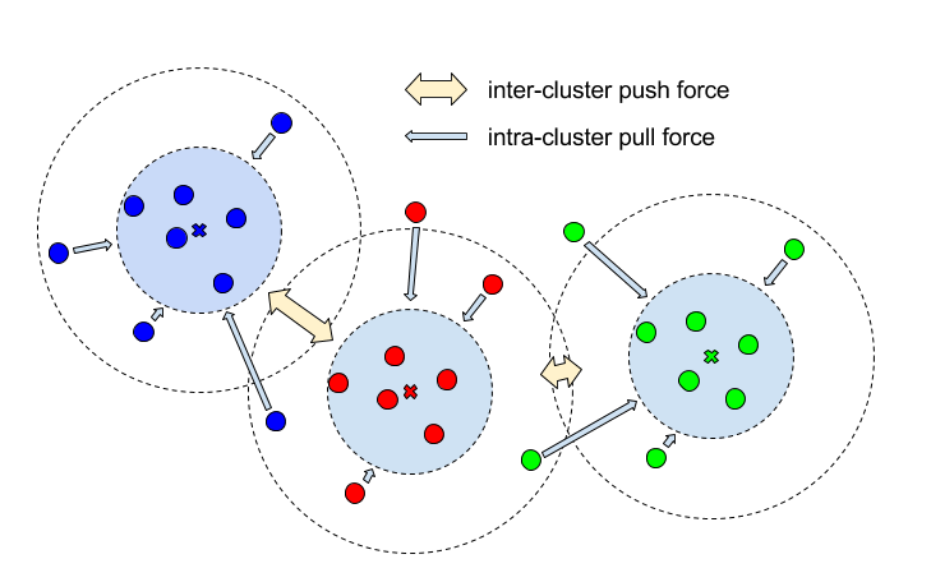
\includegraphics[width=0.5\textwidth]{figures/contrastive_loss.png}
	\caption{As defined by the loss, this are the hinged inter-pulling and intra-pushing forces acting on points in the embedding space \cite{brab2017semantic}}
	\label{fig_contrastive}
\end{figure}

\subsection{Triplet loss}\label{loss_triplet}
This loss, as defined in \cite{Schroff_2015} is related to the contrastive loss in section \ref{loss_contrastive} in the sense that it is also defined over data points in an embedding space where the resulting embeddings form ideally per instance clusters. The loss function expects three embedding vectors as an input. An anchor $x_i^a$, a embedding that is of the same class $x_i^p$ and one that is of a different class $x_i^n$. Then the loss yields

\begin{align}
	\mathcal{L}_{trpl} = \sum_i^N \left[ \norm{x_i^a - x_i^p}^2 - \norm{x_i^a - x_i^n}^2 + \alpha \right]_+ \text{\hspace{1mm}.}
\end{align} 

Again $[x]_+ = \max(0, x)$, $N$ is the number of all possible triplets $(x_i^a, x_i^p, x_i^n) \in \mathcal{T}$ in the embeddings, $\norm{\cdot}$ is the $L2$ norm and $\alpha$ is a enforced margin between positive and negative pairs. The training behavior using $\mathcal{L}_{trpl}$ as a loss is depicted in figure \ref{fig_triplet}. \\

\begin{figure}[ht!]
	\centering
	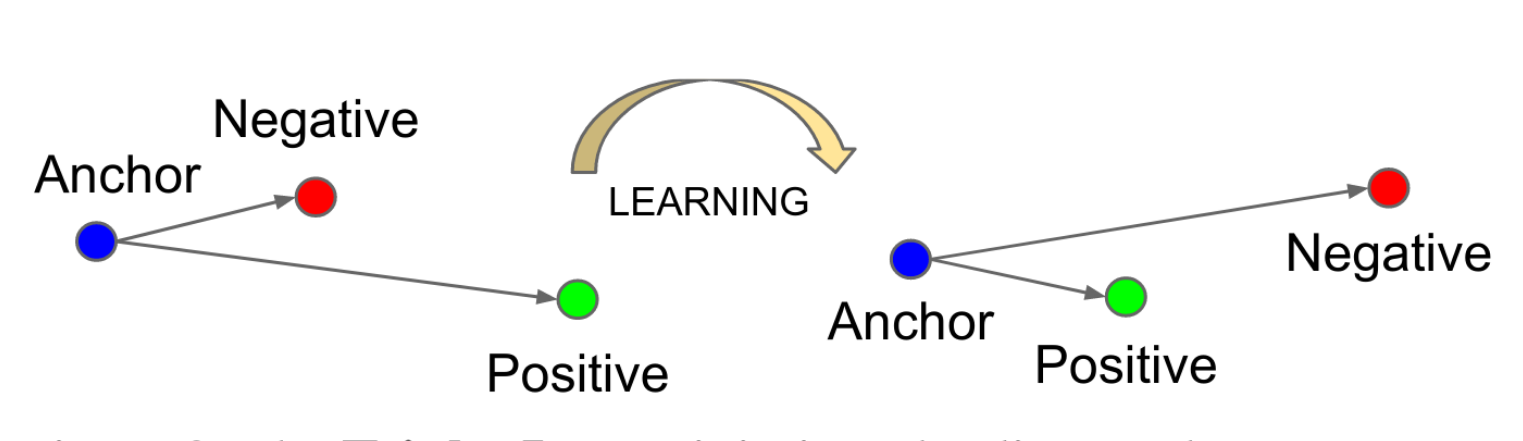
\includegraphics[width=0.5\textwidth]{figures/triplet_loss.png}
	\caption{Position of triplets in the embedding space before and after training \cite{Schroff_2015}}
	\label{fig_triplet}
\end{figure}

Often times $N$ is very large and the loss requires too many resources to calculate. Therefore it is crucial to select triples that are active, namely $\left\{ (x_i^a, x_i^p, x_i^n) \bigg| \left[ \norm{x_i^a - x_i^p}^2 - \norm{x_i^a - x_i^n}^2 + \alpha \right]_+ \neq 0 \right\}$ . However different selection strategies end in very different results regarding training time and convergence to satisfactory optima. E.g. picking only triplets that produce a high loss value can result in a training converging quickly into bad local optima.
To prevent the embeddings from diverging a regularizer term is added in order to constrain the embedding vectors to the unit hypersphere surface.
\begin{align}
	\mathcal{L}_{reg} = \sum_i^M\frac{1}{2}(\norm{x_i} - 1)^2
\end{align}

Here $M$ is the number of pixels in the image. The final loss therefore yields

\begin{align}
\mathcal{L} = \mathcal{L}_{trpl} + \beta \mathcal{L}_{reg}
\end{align}

where $\beta$ is a scalar weight for the regularizer term.